\flushbottom


%% CONTINUE:
%% Derive the general solution of the Bernoulli equation in an exercise.
%% Show this result in Result.



%%=============================================================================
%%=============================================================================
\chapter{Techniques for Nonlinear Differential Equations}


In mathematics you don't understand things. You just get used to them.

\begin{flushright}
  - Johann von Neumann
\end{flushright}





%%=============================================================================
\section{Bernoulli Equations}
\index{Bernoulli equations}


Sometimes it is possible to solve a nonlinear equation by
making a change of the dependent variable that converts it into a
linear equation.  One of the most important such equations is the
\textit{Bernoulli equation}
\[
\frac{\dd y}{\dd t} + p(t) y = q(t) y^\alpha, \quad \alpha \neq 1.
\]
The change of dependent variable $u = y^{1-\alpha}$ will yield a first order linear
equation for $u$ which when solved will give us an
implicit solution for $y$.  (See Exercise~\ref{exercise t2dydt+2ty-y3=0}.)




\begin{Result}
  The Bernoulli equation $y' + p(t) y = q(t) y^\alpha,\ \alpha \neq 1$ can 
  be transformed to the first order linear equation
  \[
  \frac{\dd u}{\dd t} + (1-\alpha) p(t) u = (1 - \alpha) q(t)
  \]
  with the change of variables $u = y^{1-\alpha}$.
\end{Result}







\begin{Example}
  Consider the Bernoulli equation
  \begin{gather*}
    y' = \frac{2}{x} y + y^2. \\
    \intertext{First we divide by $y^2$.}
    y^{-2}y' = \frac{2}{x} y^{-1} + 1 \\
    \intertext{We make the change of variable $u = y^{-1}$.}
    -u' = \frac{2}{x} u + 1 \\
    u' + \frac{2}{x} u = -1 \\
    \intertext{The integrating factor is 
      $I(x) = \exp(\int \frac{2}{x}\,d x) = x^2$.}
    \frac{d}{d x}(x^2 u) = -x^2 \\
    x^2 u = -\frac{1}{3} x^3 + c \\
    u = -\frac{1}{3} x + \frac{c}{x^2} \\
    y = \left(-\frac{1}{3} x + \frac{c}{x^2} \right)^{-1}
    \intertext{Thus the solution for $y$ is}
    \boxed{
      y = \frac{ 3 x^2 }{ c - x^2 }.
      }
  \end{gather*}
\end{Example}






%%============================================================================
\section{Riccati Equations}
\index{Riccati equations}

\paragraph{Factoring Second Order Operators.}
Consider the second order linear equation
\[L[y] = \left[\frac{\dd^2}{\dd x^2} + p(x) \frac{\dd}{\dd x} + q(x) \right] y = 
y'' + p(x) y' + q(x) y = f(x).\]
If we were able to factor the linear operator $L$ into the form
\begin{equation}
  \label{eqn_factored}
  L = \left[\frac{\dd}{\dd x} + a(x) \right]\left[\frac{\dd}{\dd x} + b(x)\right],
\end{equation}
then we would be able to solve the differential equation.  Factoring
reduces the problem to a system of first order equations.  We start with the
factored equation
\[\left[\frac{\dd}{\dd x} + a(x) \right]\left[\frac{\dd}{\dd x} + b(x)\right] y
= f(x).\]
We set $u = \left[\frac{\dd}{\dd x} + b(x)\right] y$ and solve the problem
\[ \left[\frac{\dd}{\dd x} + a(x) \right] u = f(x).\]
Then to obtain the solution we solve
\[\left[\frac{\dd}{\dd x} + b(x)\right] y = u.\]


\begin{Example}
  Consider the equation
  \[y'' + \left(x - \frac{1}{x}\right)y' + \left(\frac{1}{x^2} - 1\right)y=0.\]
  Let's say by some insight or just random luck we are able to see that 
  this equation can be factored into
  \[ \left[\frac{\dd}{\dd x} + x \right]\left[\frac{\dd}{\dd x} - \frac{1}{x} \right]y=0.\]
  We first solve the equation
  \begin{gather*}
    \left[\frac{\dd}{\dd x} + x \right] u = 0. \\
    u' + x u = 0 \\
    \frac{\dd}{\dd x} \left(\e^{x^2/2} u\right) = 0 \\
    u = c_1 \e^{-x^2/2}
  \end{gather*}
  Then we solve for $y$ with the equation
  \begin{gather*}
    \left[\frac{\dd}{\dd x} - \frac{1}{x} \right]y = u = c_1 \e^{-x^2/2}. \\
    y' - \frac{1}{x} y = c_1 \e^{-x^2/2} \\
    \frac{\dd}{\dd x} \left(x^{-1} y\right) = c_1 x^{-1} \e^{-x^2/2} \\
    \boxed{y = c_1 x \int x^{-1} \e^{-x^2/2}\,d x + c_2 x}
  \end{gather*}
\end{Example}


If we were able to solve for $a$ and $b$ 
in Equation~\ref{eqn_factored} in terms of $p$ and $q$
then we would be able to solve any second order differential equation.  
Equating the two operators, 
\begin{align*}
  \frac{\dd^2}{\dd x^2} + p \frac{\dd}{\dd x} + q 
  &= \left[\frac{\dd}{\dd x} + a \right]
  \left[\frac{\dd}{\dd x} + b\right] \\
  &= \frac{\dd^2}{\dd x^2} + (a + b)\frac{\dd}{\dd x} 
  + (b' + a b).
\end{align*}
Thus we have the two equations
\[ a + b = p, \quad \mathrm{and} \quad 
b' + a b = q. \]
Eliminating $a$, 
\begin{gather*}
  b' + (p - b) b = q \\
  b' = b^2 - p b + q
\end{gather*}
Now we have a nonlinear equation for $b$ 
that is no easier to solve than the original
second order linear equation.

\paragraph{Riccati Equations.}
Equations of the form
\[ y' = a(x) y^2 + b(x) y + c(x)\]
are called Riccati equations.  From the above derivation we see that for
every second order differential equation there is a corresponding Riccati
equation.  Now we will show that the converse is true.

We make the substitution 
\[y = -\frac{u'}{au}, \qquad 
y' = -\frac{u''}{a u} + \frac{(u')^2}{a u^2} 
+ \frac{a' u'}{a^2 u}, \]
in the Riccati equation.
\begin{gather*}
  y' = a y^2 + b y + c \\
  -\frac{u''}{a u} + \frac{(u')^2}{a u^2} 
  + \frac{a' u'}{a^2 u}
  = a \frac{(u')^2}{a^2 u^2} - b \frac{u'}{a u}+c\\
  -\frac{u''}{a u} + \frac{a' u'}{a^2 u} + b \frac{u'}{a u}
  - c = 0 \\
  u'' - \left(\frac{a'}{a} + b\right) u'+ a c u = 0
\end{gather*}
Now we have a second order linear equation for $u$.



\begin{Result}
  The substitution $y = -\frac{u'}{a u}$ transforms the Riccati 
  equation
  \[
  y' = a(x) y^2 + b(x) y + c(x)
  \]
  into the second order linear equation
  \[
  u'' - \left(\frac{a'}{a} + b\right) u'+ a c u = 0.
  \]
\end{Result}




\begin{Example}
  Consider the Riccati equation
  \[ y' = y^2 + \frac{1}{x} y + \frac{1}{x^2}. \]
  With the substitution $y = -\frac{u'}{u}$ we obtain
  \[ u'' - \frac{1}{x} u' + \frac{1}{x^2} u = 0. \]
  This is an Euler equation.  The substitution $u = x^\lambda$ yields
  \[ \lambda(\lambda-1) - \lambda + 1 = (\lambda-1)^2 = 0. \]
  Thus the general solution for $u$ is
  \[ u = c_1 x + c_2 x \log x. \]
  Since $y = -\frac{u'}{u}$,
  \begin{gather*} 
    y = -\frac{c_1 + c_2 (1 + \log x)}{c_1 x + c_2 x \log x} \\
    \boxed{
      y = -\frac{1 + c (1 + \log x)}{x + c x \log x} 
      }
  \end{gather*}
\end{Example}









%%============================================================================
\section{Exchanging the Dependent and Independent Variables}
\index{exchanging dep. and indep. var.}



Some differential equations can be put in a more elementary form by
exchanging the dependent and independent variables.  If the new equation can
be solved, you will have an implicit solution for the initial
equation. We will consider a few
examples to illustrate the method.




\begin{Example}
  Consider the equation
  \[ y' = \frac{1}{y^3 - x y^2}.\]
  Instead of considering $y$ to be a function of $x$,
  consider $x$ to be a function
  of $y$.  That is, $x = x(y)$, $x' = \frac{\dd x}{\dd y}$.
  \begin{gather*}
    \frac{\dd y}{\dd x} = \frac{1}{y^3 - x y^2} \\
    \frac{\dd x}{\dd y} = y^3 - x y^2 \\
    x' + y^2 x = y^3 \\
    \intertext{Now we have a first order equation for $x$.}
    \frac{\dd}{\dd y} \left(\e^{y^3/3} x\right) = y^3 \e^{y^3/3} \\
    \boxed{x = \e^{-y^3/3} \int y^3 \e^{y^3/3}\,d y + c \e^{-y^3/3}}
  \end{gather*}
\end{Example}


\begin{Example}
  Consider the equation
  \[y' = \frac{y}{y^2 + 2x}.\]
  Interchanging the dependent and independent variables yields
  \begin{gather*}
    \frac{1}{x'} = \frac{y}{y^2 + 2x} \\
    x' = y + 2\frac{x}{y} \\
    x' - 2 \frac{x}{y} = y \\
    \frac{\dd}{\dd y} (y^{-2} x) = y^{-1} \\
    y^{-2} x = \log y + c \\
    \boxed{x = y^2 \log y + c y^2}
  \end{gather*}
\end{Example}





\begin{Result}
  Some differential equations can be put in a simpler form by exchanging
  the dependent and independent variables.  Thus a differential equation for
  $y(x)$ can be written as an equation for $x(y)$.  Solving the equation
  for $x(y)$ will give an implicit solution for $y(x)$.
\end{Result}











%%============================================================================
\section{Autonomous Equations}
\index{differential equations!autonomous}
\index{autonomous D.E.}
Autonomous equations have no explicit dependence on $x$.
The following are examples.
\begin{itemize}
\item $y'' + 3 y' - 2y = 0$
\item $y'' = y + (y')^2$
\item $y''' + y'' y = 0$
\end{itemize}

The change of variables $u(y) = y'$ reduces an $n^{th}$ order
autonomous equation in $y$
to a non-autonomous equation of order $n-1$ in $u(y)$.  Writing the derivatives
of $y$ in terms of $u$,
\begin{align*}
  y'      &= u(y) \\
  y''     &= \frac{\dd}{\dd x} u(y) \\
  &= \frac{\dd y}{\dd x}\frac{\dd}{\dd y} u(y) \\
  &= y' u' \\
  &= u' u \\
  y'''    &= (u'' u + (u')^2)u.
\end{align*}
Thus we see that the equation for $u(y)$ will have an order of one less than
the original equation.



\begin{Result}
  Consider an autonomous differential equation for $y(x)$, 
  (autonomous equations have no explicit dependence on $x$.)
  The change of variables $u(y) = y'$ reduces an $n^{th}$ order
  autonomous equation in $y$
  to a non-autonomous equation of order $n-1$ in $u(y)$.
\end{Result}




\begin{Example}
  Consider the equation
  \[ y'' = y + (y')^2.\]
  With the substitution $u(y) = y'$, the equation becomes
  \begin{gather*}
    u' u = y + u^2 \\
    u' = u + y u^{-1}. \\
    \intertext{We recognize this as a Bernoulli equation.  
      The substitution $v = u^2$ yields}
    \frac{1}{2} v' = v + y \\
    v' - 2v = 2y \\
    \frac{\dd}{\dd y} \left(\e^{-2y} v\right) = 2y \e^{-2y} \\
    v(y) = c_1 \e^{2y} + \e^{2y}\int 2y \e^{-2y}\,d y \\
    v(y) = c_1 \e^{2y} + \e^{2y}\left( -y \e^{-2y} + 
      \int \e^{-2y}\,d y \right) \\
    v(y) = c_1 \e^{2y} + \e^{2y}\left( -y \e^{-2y} - \frac{1}{2} \e^{-2y}\right)\\
    v(y) = c_1 \e^{2y} - y - \frac{1}{2}. \\
    \intertext{Now we solve for $u$.}
    u(y) = \left(c_1 \e^{2y} - y - \frac{1}{2}\right)^{1/2}. \\
    \frac{\dd y}{\dd x} = \left(c_1 \e^{2y} - y - \frac{1}{2}\right)^{1/2} \\
    \intertext{This equation is separable.}
    d x = \frac{d y}{\left(c_1 \e^{2y} - y - \frac{1}{2}\right)^{1/2}} \\
    \boxed{ x + c_2 = \int \frac{1}{\left(c_1 \e^{2y} - y - \frac{1}{2}
        \right)^{1/2}}\,d y }
  \end{gather*}
  Thus we finally have arrived at an implicit solution for $y(x)$.
\end{Example}




\begin{Example}
  Consider the equation
  \[y'' + y^3 = 0.\]
  With the change of variables, $u(y) = y'$, the equation becomes
  \[ u' u + y^3 = 0. \]
  This equation is separable.
  \begin{gather*}
    u\,d u = - y^3\,d y \\
    \frac{1}{2} u^2 = - \frac{1}{4} y^4 + c_1 \\
    u = \left( 2c_1 -\frac{1}{2} y^4 \right)^{1/2} \\
    y' = \left( 2c_1 -\frac{1}{2} y^4 \right)^{1/2} \\
    \frac{d y}{(2c_1 -\frac{1}{2} y^4 )^{1/2}} = d x \\
    \intertext{Integrating gives us the implicit solution}
    \boxed{ \int \frac{1}{(2c_1 -\frac{1}{2} y^4 )^{1/2}}\,d y = x + c_2 .}
  \end{gather*}
\end{Example}













%%============================================================================
\section{*Equidimensional-in-x Equations}
\index{differential equations!equidimensional-in-x}
\index{equidimensional-in-x D.E.} 

Differential equations that are invariant under the change of variables
$x = c\,\xi$
are said to be equidimensional-in-$x$.  
For a familiar example from linear equations, we note that 
the Euler equation is 
equidimensional-in-$x$.  Writing the new derivatives under the change of 
variables,
\[ x = c\,\xi, \qquad \frac{\dd}{\dd x} = \frac{1}{c} \frac{\dd}{\dd \xi}, \qquad
\frac{\dd^2}{\dd x^2} = \frac{1}{c^2}\frac{\dd^2}{\dd \xi^2}, \qquad \ldots.\]




\begin{Example}
  Consider the Euler equation
  \[ y'' + \frac{2}{x} y' + \frac{3}{x^2}y = 0.\]
  Under the change of variables, $x = c\,\xi$, $y(x) = u(\xi)$,
  this equation becomes
  \begin{gather*}
    \frac{1}{c^2} u'' + \frac{2}{c\,\xi} \frac{1}{c}u'
    + \frac{3}{c^2\,\xi^2} u = 0 \\
    u'' + \frac{2}{\xi} u' + \frac{3}{\xi^2}u = 0.
  \end{gather*}
  Thus this equation is invariant under the change of variables $x = c\,\xi$.
\end{Example}



\begin{Example} \label{nonlin_equidim}
  For a nonlinear example, consider the equation
  \[ y''\,y' + \frac{y''}{x\,y}+ \frac{y'}{x^2} = 0.\]
  With the change of variables $x = c\,\xi$, $y(x) = u(\xi)$
  the equation becomes
  \begin{gather*}
    \frac{u''}{c^2}\frac{u'}{c} + \frac{u''}{c^3\,\xi\,u} 
    + \frac{u'}{c^3\,\xi^2} = 0 \\
    u''\,u' + \frac{u''}{\xi\,u} 
    + \frac{u'}{\xi^2} = 0.
  \end{gather*}
  We see that this equation is also equidimensional-in-$x$.
\end{Example}




You may recall that the change of variables $x = \e^t$ reduces an Euler
equation to a constant coefficient equation. 
To generalize this result to nonlinear equations we will see that the
same change of variables reduces an equidimensional-in-$x$ equation to
an autonomous equation.

Writing the derivatives with respect to $x$ in terms of $t$,
\[
x = \e^t, \qquad
\frac{\dd}{\dd x} = \frac{\dd t}{\dd x} \frac{\dd}{\dd t} = \e^{-t}\frac{\dd}{\dd t} 
\]
\[
x\frac{\dd}{\dd x} = \frac{\dd}{\dd t}
\]
\[
x^2 \frac{\dd^2}{\dd x^2} = x \frac{\dd}{\dd x} \left(x \frac{\dd}{\dd x}\right) 
- x\frac{\dd}{\dd x} = \frac{\dd^2}{\dd t^2} - \frac{\dd}{\dd t}.
\]


\begin{Example} 
  Consider the equation in Example~\ref{nonlin_equidim} 
  \[ y''\,y' + \frac{y''}{x\,y}+ \frac{y'}{x^2} = 0.\]
  Applying the change of variables $x = \e^t$, $y(x) = u(t)$ yields an 
  autonomous equation for $u(t)$.
  \begin{gather*}
    x^2\,y''\,x\,y' + \frac{x^2\,y''}{y} + x\,y' = 0 \\
    \boxed{ (u'' - u') u' + \frac{u'' - u'}{u} + u' = 0  }
  \end{gather*}
\end{Example}







\begin{Result}
  A differential equation that is invariant under the change of variables
  $x = c\,\xi$ is equidimensional-in-$x$.  Such an equation can be reduced
  to autonomous equation of the same order with the change of variables,
  $x = \e^t$.
\end{Result}














%%============================================================================
\section{*Equidimensional-in-y Equations}
\index{differential equations!equidimensional-in-y}
\index{equidimensional-in-y D.E.}
A differential equation is said to be equidimensional-in-$y$ if it is invariant
under the change of variables $y(x) = c\,v(x)$.  Note that all linear
homogeneous equations are equidimensional-in-$y$.





\begin{Example} \label{lin_eiy} 
  Consider the linear equation
  \[ y'' + p(x) y' + q(x) y = 0.\]
  With the change of variables $y(x) = c v(x)$ the equation becomes
  \begin{gather*}
    c v'' + p(x)c v' + q(x) c v = 0 \\
    v'' + p(x)v' + q(x) v = 0
  \end{gather*}
  Thus we see that the equation is invariant under the change of variables.
\end{Example}








\begin{Example} \label{nonlin_eiy}
  For a nonlinear example, consider the equation
  \[ y'' y + (y')^2 - y^2 = 0.\]
  Under the change of variables $y(x) = c v(x)$ the equation becomes.
  \begin{gather*}
    c v'' c v + (c v')^2 - (c v)^2 = 0 \\
    v'' v + (v')^2 - v^2 = 0.
  \end{gather*}
  Thus we see that this equation is also equidimensional-in-$y$.
\end{Example}



The change of variables $y(x) = \e^{u(x)}$ reduces an $n^{t h}$ order
equidimensional-in-$y$ equation to an equation of order $n-1$ for $u'$.
Writing the derivatives of $\e^{u(x)}$,
\begin{align*}
  \frac{\dd}{\dd x} \e^u &= u' \e^u \\
  \frac{\dd^2}{\dd x^2} \e^u &= (u'' + (u')^2)\e^u \\
  \frac{d^3}{d x^3}\e^u &= (u''' + 3u'' u'' + (u')^3)\e^u.
\end{align*}


\begin{Example}
  Consider the linear equation in Example~\ref{lin_eiy} 
  \[ y'' + p(x) y' + q(x) y = 0.\]
  Under the change of variables $y(x) = \e^{u(x)}$ the equation becomes
  \begin{gather*}
    (u'' + (u')^2)\e^u + p(x) u' \e^u + q(x) \e^u = 0 \\
    \boxed{ u'' + (u')^2 + p(x) u' + q(x) = 0. }
  \end{gather*}
  Thus we have a Riccati  equation for $u'$.  
  This transformation might seem rather useless since linear equations are usually
  easier to work with than nonlinear equations, but it is often useful in determining
  the asymptotic behavior of the equation.
\end{Example}





\begin{Example}
  From Example~\ref{nonlin_eiy} we have the equation
  \[ y'' y + (y')^2 - y^2 = 0.\]
  The change of variables $y(x) = \e^{u(x)}$ yields
  \begin{gather*}
    (u'' + (u')^2) \e^u \e^u + (u' \e^u)^2 - (\e^u)^2 = 0 \\
    u'' + 2(u')^2 - 1 = 0 \\
    u'' = -2 (u')^2 + 1 
  \end{gather*}
  Now we have a Riccati equation for $u'$.  
  We make the substitution $u' = \frac{v'}{2 v}$.
  \begin{gather*}
    \frac{v''}{2v} - \frac{(v')^2}{2v^2} = - 2 \frac{(v')^2}{4v^2} + 1 \\
    v'' - 2 v = 0 \\
    v = c_1 \e^{\sqrt{2} x} + c_2 \e^{-\sqrt{2} x} \\
    u' = 2 \sqrt{2} \frac{c_1 \e^{\sqrt{2} x} - c_2 \e^{-\sqrt{2} x}}
    {c_1 \e^{\sqrt{2} x} + c_2 \e^{-\sqrt{2} x}} \\
    u = 2 \int \frac{c_1 \sqrt{2} \e^{\sqrt{2} x} 
      - c_2 \sqrt{2} \e^{-\sqrt{2} x}}
    {c_1 \e^{\sqrt{2} x} + c_2 \e^{-\sqrt{2} x}} \,d x + c_3 \\
    u = 2 \log \left( c_1 \e^{\sqrt{2} x} + c_2 \e^{-\sqrt{2} x} \right) + c_3 \\
    y = \left( c_1 \e^{\sqrt{2} x} + c_2 \e^{-\sqrt{2} x} \right)^2 \e^{c_3}
  \end{gather*}
  The constants are redundant, the general solution is
  \[
  \boxed{
    y = \left( c_1 \e^{\sqrt{2} x} + c_2 \e^{-\sqrt{2} x} \right)^2
    }
  \]
\end{Example}




\begin{Result}
  A differential equation is equidimensional-in-$y$ if it is invariant under 
  the change of variables $y(x) = c v(x)$.  An $n^{t h}$ order 
  equidimensional-in-$y$ equation can be reduced to an equation of order 
  $n-1$ in $u'$ with the change of variables $y(x) = \e^{u(x)}$.
\end{Result}











%%============================================================================
\section{*Scale-Invariant Equations}
\index{differential equations!scale-invariant}
\index{scale-invariant D.E.}



\begin{Result}
  An equation is scale invariant if it is invariant under the change of 
  variables, $x = c\xi$, $y(x) = c^\alpha v(\xi)$, for some value of $\alpha$.
  A scale-invariant equation can be transformed to an equidimensional-in-$x$
  equation with the change of variables, $y(x) = x^\alpha u(x)$.
\end{Result}







\begin{Example}
  Consider the equation
  \[ y'' + x^2 y^2 = 0.\]
  Under the change of variables $x = c\xi$, $y(x) = c^\alpha v(\xi)$ this
  equation becomes
  \[ \frac{c^\alpha}{c^2}v''(\xi) + c^2 x^2 c^{2\alpha} v^2(\xi) = 0.\]
  Equating powers of $c$ in the two terms yields $\alpha = -4$.  

  Introducing the change of variables $y(x) = x^{-4}u(x)$ yields
  \begin{gather*}
    \frac{\dd^2}{\dd x^2} \big[ x^{-4}u(x) \big] + x^2 (x^{-4}u(x))^2 = 0 \\
    x^{-4}u'' - 8 x^{-5}u' + 20 x^{-6}u + x^{-6}u^2 = 0 \\
    \boxed{ x^2 u'' - 8 x u' + 20 u + u^2 = 0. }
  \end{gather*}
  We see that the equation for $u$ is equidimensional-in-$x$.
\end{Example}











\raggedbottom
%%==========================================================================
\exercises{
\pagebreak
\flushbottom
\section{Exercises}






%% CONTINUE: add a Clairaut section.
%% y = x p + p^2.
\begin{Exercise}
  \label{exercise y=xp+p2}
  \begin{enumerate}
  \item
    Find the general solution and the singular solution of the Clairaut equation,
    \[
    y = x p + p^2.
    \]
  \item
    Show that the singular solution is the envelope of the general solution.
  \end{enumerate}

  \hintsolution{y=xp+p2}
\end{Exercise}





%%-----------------------------------------------------------------------------
\begin{large}
  \noindent
  \textbf{Bernoulli Equations}
\end{large}






%% \frac{\dd y}{\dd t} + p(t) y = q(t) y^\alpha.
\begin{Exercise}[mathematica/ode/techniques\_nonlinear/bernoulli.nb]
  \label{exercise dydt+py=qy}
  Consider the Bernoulli equation
  \[
  \frac{\dd y}{\dd t} + p(t) y = q(t) y^\alpha.
  \]
  \begin{enumerate}
  \item
    Solve the Bernoulli equation for $\alpha = 1$.
  \item
    Show that for $\alpha \neq 1$ the substitution $u = y^{1-\alpha}$ reduces 
    Bernoulli's equation to a linear equation.
  \item
    Find the general solution to the following equations.
    \begin{enumerate}
    \item 
      \centerline{$\displaystyle t^2 \frac{\dd y}{\dd t} + 2 t y - y^3 = 0,\ t > 0$}
    \item 
      \centerline{$\displaystyle \frac{\dd y}{\dd x} + 2 x y + y^2 = 0$}
    \end{enumerate}
  \end{enumerate}

  \hintsolution{dydt+py=qy}
\end{Exercise}





%% Consider a population, $y$.  Let the birth rate of the population be 
\begin{Exercise}
  \label{exercise population}
  Consider a population, $y$.  Let the birth rate of the population be 
  proportional to $y$ with constant of proportionality $1$.  Let the death
  rate of the population be proportional to $y^2$ with constant of 
  proportionality $1/1000$.  Assume that the population is large enough
  so that you can consider $y$ to be continuous.  What is the population as
  a function of time if the initial population is $y_0$?

  \hintsolution{population}
\end{Exercise}




%% t^2 \frac{\dd y}{\dd t} + 2 t y - y^3 = 0 \quad t > 0
\begin{Exercise}
  \label{exercise t2dydt+2ty-y3=0}
  Show that the transformation $u = y^{1-n}$
  reduces the equation to a linear first order equation.  Solve the equations
  \begin{enumerate}
  \item
    $
    \displaystyle
    t^2 \frac{\dd y}{\dd t} + 2 t y - y^3 = 0 \quad t > 0
    $
  \item
    $
    \displaystyle
    \frac{\dd y}{\dd t} = \left( \Gamma \cos t + T \right) y - y^3,
    $
    $\Gamma$ and $T$ are real constants.  (From a fluid flow stability problem.)
  \end{enumerate}

  \hintsolution{t2dydt+2ty-y3=0}
\end{Exercise}





%%-----------------------------------------------------------------------------
\begin{large}
  \noindent
  \textbf{Riccati Equations}
\end{large}






%% Riccati equations, two methods of solution.
\begin{Exercise}
  \label{exercise riccati 2 methods}
  \begin{enumerate}
    %%
    %%
  \item
    Consider the Ricatti equation,
    \[
    \frac{\dd y}{\dd x} = a(x) y^2 + b(x) y + c(x).
    \]
    Substitute 
    \[
    y = y_p(x) + \frac{1}{u(x)}
    \]
    into the Ricatti equation, where $y_p$ is some particular solution to obtain
    a first order linear differential equation for $u$.
    %%
    %%
  \item
    Consider a Ricatti equation,
    \[
    y' = 1 + x^2 - 2 x y + y^2.
    \]
    Verify that $y_p(x) = x$ is a particular solution.
    Make the substitution $y = y_p + 1/u$ to find the general solution.

    What would happen if you continued this method, taking the general solution
    for $y_p$?  Would you be able to find a more general solution?
    %%
    %%
  \item
    The substitution
    \[
    y = - \frac{u'}{a u}
    \]
    gives us the second order, linear, homogeneous differential equation,
    \[
    u'' - \left( \frac{a'}{a} + b \right) u' + a c u = 0.
    \]
    The general solution for $u$ has two constants of integration.  However, the 
    solution for $y$ should only have one constant of integration as it satisfies
    a first order equation.  Write $y$ in terms of the solution for $u$ and verify
    tha $y$ has only one constant of integration.
  \end{enumerate}

  \hintsolution{riccati 2 methods}
\end{Exercise}






%%-----------------------------------------------------------------------------
\begin{large}
  \noindent
  \textbf{Exchanging the Dependent and Independent Variables}
\end{large}













%% Solve the differential equation \[ y' = \frac{\sqrt{y}}{x y + y}.\]
\begin{Exercise}
  \label{exercise y'=sqrt y xyy}
  Solve the differential equation
  \[
  y' = \frac{\sqrt{y}}{x y + y}.
  \]

  \hintsolution{y'=sqrt y xyy}
\end{Exercise}



%%-----------------------------------------------------------------------------
\begin{large}
  \noindent
  \textbf{Autonomous Equations}
\end{large}



%%-----------------------------------------------------------------------------
\begin{large}
  \noindent
  \textbf{*Equidimensional-in-$\mathbf{x}$ Equations}
\end{large}



%%-----------------------------------------------------------------------------
\begin{large}
  \noindent
  \textbf{*Equidimensional-in-$\mathbf{y}$ Equations}
\end{large}



%%-----------------------------------------------------------------------------
\begin{large}
  \noindent
  \textbf{*Scale-Invariant Equations}
\end{large}







\raggedbottom
}
%%==========================================================================
\hints{
\pagebreak
\flushbottom
\section{Hints}





%% y = x p + p^2.
\begin{Hint}
  \label{hint y=xp+p2}
  %% CONTINUE
\end{Hint}






%%-----------------------------------------------------------------------------
\begin{large}
  \noindent
  \textbf{Bernoulli Equations}
\end{large}





%% \frac{\dd y}{\dd t} + p(t) y = q(t) y^\alpha.
\begin{Hint}
  \label{hint dydt+py=qy}
  %% CONTINUE
\end{Hint}





%% Consider a population, $y$.  Let the birth rate of the population be 
\begin{Hint}
  \label{hint population}
  The differential equation governing the population is
  \[ 
  \frac{\dd y}{\dd t} = y - \frac{y^2}{1000}, \quad y(0) = y_0. 
  \]
  This is a Bernoulli equation.
\end{Hint}





%% t^2 \frac{\dd y}{\dd t} + 2 t y - y^3 = 0 \quad t > 0
\begin{Hint}
  \label{hint t2dydt+2ty-y3=0}
  %% CONTINUE
\end{Hint}



%%-----------------------------------------------------------------------------
\begin{large}
  \noindent
  \textbf{Riccati Equations}
\end{large}





%% Riccati equations, two methods of solution.
\begin{Hint}
  \label{hint riccati 2 methods}
  %% CONTINUE
\end{Hint}







%%-----------------------------------------------------------------------------
\begin{large}
  \noindent
  \textbf{Exchanging the Dependent and Independent Variables}
\end{large}



%% Solve the differential equation \[ y' = \frac{\sqrt{y}}{x y + y}.\]
\begin{Hint}
  \label{hint y'=sqrt y xyy}
  Exchange the dependent and independent variables.
\end{Hint}



%%-----------------------------------------------------------------------------
\begin{large}
  \noindent
  \textbf{Autonomous Equations}
\end{large}



%%-----------------------------------------------------------------------------
\begin{large}
  \noindent
  \textbf{*Equidimensional-in-$\mathbf{x}$ Equations}
\end{large}



%%-----------------------------------------------------------------------------
\begin{large}
  \noindent
  \textbf{*Equidimensional-in-$\mathbf{y}$ Equations}
\end{large}



%%-----------------------------------------------------------------------------
\begin{large}
  \noindent
  \textbf{*Scale-Invariant Equations}
\end{large}








\raggedbottom
}
%%===========================================================================
\solutions{
\pagebreak
\flushbottom
\section{Solutions}







%% y = x p + p^2.
\begin{Solution}
  \label{solution y=xp+p2}
  We consider the Clairaut equation,
  \begin{equation}
    \label{a_clairaut_eqn}
    y = x p + p^2.
  \end{equation}

  \begin{enumerate}
    %%
    %%
  \item
    We differentiate Equation~\ref{a_clairaut_eqn} with respect to $x$ to obtain
    a second order differential equation.
    \begin{gather*}
      y' = y' + x y'' + 2 y' y'' \\
      y'' (2y' + x) = 0
    \end{gather*}
    Equating the first or second factor to zero will lead us to two distinct
    solutions.
    \[
    y'' = 0 \quad \mathrm{or} \quad y' = - \frac{x}{2}
    \]
    If $y'' = 0$ then $y' \equiv p$ is a constant, (say $y' = c$).  From 
    Equation~\ref{a_clairaut_eqn} we see that the general solution is,
    \begin{equation}
      \label{clairaut_first_soln}
      \boxed{
        y(x)  = c x + c^2.
        }
    \end{equation}
    Recall that the general solution of a first order differential equation 
    has one constant of integration.

    If $y' = - x / 2$ then $y = -x^2 / 4 + \mathrm{const}$.  We determine the 
    constant by substituting the expression into Equation~\ref{a_clairaut_eqn}.
    \[
    - \frac{x^2}{4} + c = x \left( - \frac{x}{2} \right) + \left( - \frac{x}{2} 
    \right)^2
    \]
    Thus we see that a singular solution of the Clairaut equation is
    \begin{equation}
      \label{clairaut_second_soln}
      \boxed{
        y(x) = - \frac{1}{4} x^2.
        }
    \end{equation}
    Recall that a singular solution of a first order nonlinear differential 
    equation has no constant of integration.
    %%
    %%
  \item
    Equating the general and singular solutions, $y(x)$, and their derivatives, 
    $y'(x)$, gives us the system of equations,
    \[
    c x + c^2 = - \frac{1}{4} x^2, \qquad c = - \frac{1}{2} x.
    \]
    Since the first equation is satisfied for $c = - x / 2$, we see that 
    the solution $y = c x + c^2$ is tangent to the solution $y = - x^2 / 4$
    at the point $(-2 c, -|c|)$.
    The solution $y = c x + c^2$ is plotted for $c = \ldots,-1/4,0,1/4,\ldots$
    in Figure~\ref{clairaut_envelope}.

    \begin{figure}[tb!]
      \begin{center}
        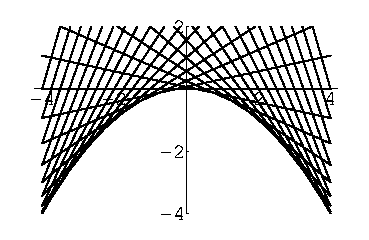
\includegraphics[width=0.4\textwidth]{ode/techniques_nonlinear/clairaut_envelope}
      \end{center}
      \caption{The solutions and their envelope.}
      \label{clairaut_envelope}
    \end{figure}

    The envelope of a one-parameter family $F(x,y,c) = 0$ is given by the 
    system of equations,
    \[
    F(x,y,c) = 0, \qquad F_c(x,y,c) = 0.
    \]
    For the family of solutions $y = c x + c^2$ these equations are
    \[
    y = c x + c^2, \qquad 0 = x + 2 c.
    \]
    Substituting the solution of the second equation, $c = - x/2$, into the
    first equation gives the envelope,
    \[
    y = \left( - \frac{1}{2} x \right) x + \left( - \frac{1}{2} x \right)^2
    = - \frac{1}{4} x^2.
    \]
    Thus we see that the singular solution is the envelope of the general solution.
  \end{enumerate}
\end{Solution}







%%-----------------------------------------------------------------------------
\begin{large}
  \noindent
  \textbf{Bernoulli Equations}
\end{large}







%% \frac{\dd y}{\dd t} + p(t) y = q(t) y^\alpha.
\begin{Solution}
  \label{solution dydt+py=qy}
  \begin{enumerate}
    %%
    %%
  \item
    \begin{gather*}
      \frac{\dd y}{\dd t} + p(t) y = q(t) y \\
      \frac{\dd y}{ y } = (q - p) \,\dd t \\
      \ln y = \int(q - p) \,\dd t + c \\
      \boxed{
        y = c \e^{\int (q - p) \,\dd t}
        }
    \end{gather*}
    %%
    %%
  \item
    We consider the Bernoulli equation,
    \[
    \frac{\dd y}{\dd t} + p(t) y = q(t) y^\alpha, \quad \alpha \neq 1.
    \]
    We divide by $y^\alpha$.
    \[ 
    y^{-\alpha} y' + p(t) y^{1-\alpha} = q(t) 
    \]
    This suggests the change of dependent variable $u = y^{1-\alpha}$,
    $u' = (1-\alpha)y^{-\alpha} y'$.
    \begin{gather*}
      \frac{1}{1-\alpha} \frac{\dd}{\dd t} y^{1-\alpha} + p(t) y^{1-\alpha} = q(t) \\
      \frac{\dd u}{\dd t} + (1-\alpha) p(t) u = (1 - \alpha) q(t)
    \end{gather*}
    Thus we obtain a linear equation for $u$ which when solved will give us an
    implicit solution for $y$.
    %%
    %%
  \item
    \begin{enumerate}
    \item
      \begin{gather*}
        t^2 \frac{\dd y}{\dd t} + 2 t y - y^3 = 0, \quad t > 0 \\
        t^2 \frac{ y' }{ y^3 } + 2 t \frac{ 1 }{ y^2 } = 1
      \end{gather*}
      We make the change of variables $u = y^{-2}$.
      \begin{gather*}
        - \frac{1}{2} t^2 u' + 2 t u = 1 \\
        u' - \frac{4}{t} u = - \frac{2}{t^2}
      \end{gather*}
      The integrating factor is
      \[
      \mu = \e^{\int (-4/t)\,\dd t} = \e^{-4 \ln t} = t^{-4}.
      \]
      We multiply by the integrating factor and integrate to obtain the solution.
      \begin{gather*}
        \frac{\dd}{\dd t} \left( t^{-4} u \right) = -2 t^{-6} \\
        u = \frac{2}{5} t^{-1} + c t^4 \\
        y^{-2} = \frac{2}{5} t^{-1} + c t^4 \\
        y = \pm \frac{1}{ \sqrt{ \frac{2}{5} t^{-1} + c t^4 } }
        \boxed{
          y = \pm \frac{\sqrt{5 t}}{ \sqrt{ 2 + c t^5 } }
          }
      \end{gather*}
      %%
    \item
      \begin{gather*}
        \frac{\dd y}{\dd x} + 2 x y + y^2 = 0 \\
        \frac{y'}{y^2} + \frac{2 x}{y} = -1
      \end{gather*}
      We make the change of variables $u = y^{-1}$.
      \[
      u' - 2 x u = 1
      \]
      The integrating factor is
      \[
      \mu = \e^{\int (-2 x) \,\dd x} = \e^{-x^2}.
      \]
      We multiply by the integrating factor and integrate to obtain the solution.
      \begin{gather*}
        \frac{\dd}{\dd x} \left( \e^{-x^2} u \right) = \e^{-x^2} \\
        u = \e^{x^2} \int \e^{-x^2} \,\dd x + c \e^{x^2} \\
        \boxed{
          y = \frac{ \e^{-x^2} }{ \int \e^{-x^2} \,\dd x + c }
          }
      \end{gather*}
    \end{enumerate}
  \end{enumerate}
\end{Solution}







%% Consider a population, $y$.  Let the birth rate of the population be 
\begin{Solution}
  \label{solution population}
  The differential equation governing the population is
  \[ 
  \frac{\dd y}{\dd t} = y - \frac{y^2}{1000}, \qquad y(0) = y_0.
  \]
  We recognize this as a Bernoulli equation.  The substitution $u(t) = 1/y(t)$
  yields
  \begin{gather*}
    -\frac{\dd u}{\dd t} = u - \frac{1}{1000}, \quad u(0) = \frac{1}{y_0}.\\
    u' + u = \frac{1}{1000} \\
    u = \frac{1}{y_0} \e^{-t} + \frac{\e^{-t}}{1000}\int_0^t \e^{\tau}\,d\tau\\
    u = \frac{1}{1000} + \left(\frac{1}{y_0} - \frac{1}{1000}\right)\e^{-t} \\
    \intertext{Solving for $y(t)$,}
    \boxed{
      y(t) = \left(\frac{1}{1000} + \left(\frac{1}{y_0} 
          - \frac{1}{1000}\right)\e^{-t}\right)^{-1}.
      }
  \end{gather*}
  As a check, we see that as $t \to \infty$, $y(t) \to 1000$, which is 
  an equilibrium solution of the differential equation.
  \[ 
  \frac{\dd y}{\dd t} = 0 = y - \frac{y^2}{1000} \quad \to \quad y = 1000.
  \]
\end{Solution}





%% t^2 \frac{\dd y}{\dd t} + 2 t y - y^3 = 0 \quad t > 0
\begin{Solution}
  \label{solution t2dydt+2ty-y3=0}
  \begin{enumerate}
    %%
    %%
  \item
    \begin{gather*}
      t^2 \frac{\dd y}{\dd t} + 2 t y - y^3 = 0 \\
      \frac{\dd y}{\dd t} + 2 t^{-1} y = t^{-2} y^3 \\
      \intertext{We make the change of variables $u(t) = y^{-2}(t)$.}
      u' - 4 t^{-1} u = -2 t^{-2} 
    \end{gather*}
    This gives us a first order, linear equation.  The integrating factor is
    \[
    I(t) = \e^{\int -4 t^{-1} \,d t} = \e^{-4 \log t} = t^{-4}.
    \]
    We multiply by the integrating factor and integrate.
    \begin{gather*}
      \frac{\dd}{\dd t} \left( t^{-4} u \right) = -2 t^{-6} \\
      t^{-4} u = \frac{2}{5} t^{-5} + c \\
      u = \frac{2}{5} t^{-1} + c t^4 \\
      \intertext{Finally we write the solution in terms of $y(t)$.}
      y(t) = \pm \frac{1}{ \sqrt{ \frac{2}{5} t^{-1} + c t^4 } } \\
      \boxed{
        y(t) = \pm \frac{ \sqrt{5 t} }{ \sqrt{ 2 + c t^5 } }
        }
    \end{gather*}
    %%
    %%
  \item
    \begin{gather*}
      \frac{\dd y}{\dd t} - \left( \Gamma \cos t + T \right) y = - y^3 \\
      \intertext{We make the change of variables $u(t) = y^{-2}(t)$.}
      u' + 2 \left( \Gamma \cos t + T \right) u = 2 
    \end{gather*}
    This gives us a first order, linear equation.  The integrating factor is
    \[
    I(t) = \e^{\int 2 (\Gamma \cos t + T) \,d t} = \e^{ 2 (\Gamma \sin t + T t)}
    \]
    We multiply by the integrating factor and integrate.
    \begin{gather*}
      \frac{\dd}{\dd t} \left( \e^{2 (\Gamma \sin t + T t) } u \right) 
      = 2 \e^{2 (\Gamma \sin t + T t) } \\
      u = 2 \e^{- 2 (\Gamma \sin t + T t) } \left( 
        \int \e^{2 (\Gamma \sin t + T t) } \,d t + c \right) \\
      \intertext{Finally we write the solution in terms of $y(t)$.}
      \boxed{
        y = \pm \frac{ \e^{ \Gamma \sin t + T t } }
        {\sqrt{ 2 \left( \int \e^{2 (\Gamma \sin t + T t) } \,d t + c \right)}}
        }
    \end{gather*}
  \end{enumerate}
\end{Solution}








%%-----------------------------------------------------------------------------
\begin{large}
  \noindent
  \textbf{Riccati Equations}
\end{large}


%% Riccati equations, two methods of solution.
\begin{Solution}
  \label{solution riccati 2 methods}
  We consider the Ricatti equation,
  \begin{equation}
    \label{gen_ricatti}
    \frac{\dd y}{\dd x} = a(x) y^2 + b(x) y + c(x).
  \end{equation}
  \begin{enumerate}
    %%
    %%
  \item
    We substitute 
    \[
    y = y_p(x) + \frac{1}{u(x)}
    \]
    into the Ricatti equation, where $y_p$ is some particular solution.
    \begin{gather*}
      y_p' - \frac{u'}{u^2} = 
      + a(x) \left( y_p^2 + 2 \frac{y_p}{u} + \frac{1}{u^2} \right)
      + b(x) \left( y_p + \frac{1}{u} \right) + c(x) \\
      - \frac{u'}{u^2} = b(x) \frac{1}{u} 
      + a(x) \left( 2 \frac{y_p}{u} + \frac{1}{u^2} \right) \\
      \boxed{
        u' = - \left( b + 2 a y_p \right) u - a
        }
    \end{gather*}
    We obtain a first order linear differential equation for $u$ whose solution
    will contain one constant of integration.
    %%
    %%
  \item
    We consider a Ricatti equation,
    \begin{equation}
      \label{ricatti_y1pxs}
      y' = 1 + x^2 - 2 x y + y^2.
    \end{equation}
    We verify that $y_p(x) = x$ is a solution.
    \[
    1 = 1 + x^2 - 2 x x + x^2
    \]
    Substituting $y = y_p + 1/u$ into Equation~\ref{ricatti_y1pxs} yields,
    \begin{gather*}
      u' = - \left( -2 x + 2 x \right) u - 1 \\
      u = - x + c \\
      \boxed{
        y = x + \frac{1}{c - x}
        }
    \end{gather*}

    What would happen if we continued this method?  Since $y = x + \frac{1}{c-x}$
    is a solution of the Ricatti equation we can make the substitution,
    \begin{equation}
      \label{ricatti_sub}
      y = x + \frac{1}{c-x} + \frac{1}{u(x)},
    \end{equation}
    which will lead to a solution for $y$ which has two constants of integration.
    Then we could repeat the process, substituting the sum of that solution and 
    $1/u(x)$ into the Ricatti equation to find a solution with three constants
    of integration.  We know that the general solution of a first order,
    ordinary differential equation has only one constant of integration.  
    Does this method for Ricatti equations violate this theorem?  There's only
    one way to find out.  We substitute Equation~\ref{ricatti_sub} into the 
    Ricatti equation.
    \begin{gather*}
      u' = - \left( - 2 x + 2 \left( x + \frac{1}{c - x} \right) \right) u - 1 \\
      u' = - \frac{2}{c - x} u - 1 \\
      u' + \frac{2}{c - x} u = - 1 
    \end{gather*}
    The integrating factor is 
    \[
    I(x) = \e^{2/(c-x)} = \e^{-2 \log (c-x)}
    = \frac{1}{(c-x)^2}.
    \]
    Upon multiplying by the integrating factor, the equation becomes exact.
    \begin{gather*}
      \frac{\dd}{\dd x} \left( \frac{1}{(c-x)^2} u \right) = - \frac{1}{(c-x)^2} \\
      u = (c-x)^2 \frac{-1}{c-x} + b (c-x)^2 \\
      u = x - c + b (c-x)^2
    \end{gather*}
    Thus the Ricatti equation has the solution,
    \[
    y = x + \frac{1}{c-x} + \frac{1}{x - c + b(c-x)^2}.
    \]
    It appears that we we have found a solution that has two constants of 
    integration, but appearances can be deceptive.  We do a little 
    algebraic simplification of the solution.
    \begin{gather*}
      y = x + \frac{1}{c-x} + \frac{1}{(b(c-x) - 1)(c-x)} \\
      y = x + \frac{(b(c-x) - 1) + 1}{(b(c-x) - 1)(c-x)} \\
      y = x + \frac{b}{b(c-x) - 1} \\
      y = x + \frac{1}{(c-1/b) - x} \\
    \end{gather*}
    This is actually a solution, (namely the solution we had before), with 
    one constant of integration, (namely $c - 1/b$).  Thus we see that repeated
    applications of the procedure will not produce more general solutions.
    %%
    %%
  \item
    The substitution
    \[
    y = - \frac{u'}{a u}
    \]
    gives us the second order, linear, homogeneous differential equation,
    \[
    u'' - \left( \frac{a'}{a} + b \right) u' + a c u = 0.
    \]
    The solution to this linear equation is a linear combination of two 
    homogeneous solutions, $u_1$ and $u_2$.
    \[
    u = c_1 u_1(x) + c_2 u_2(x)
    \]
    The solution of the Ricatti equation is then
    \[
    y = - \frac{ c_1 u_1'(x) + c_2 u_2'(x) }{ a(x) (c_1 u_1(x) + c_2 u_2(x)) }.
    \]
    Since we can divide the numerator and denominator by either $c_1$ or $c_2$,
    this answer has only one constant of integration, (namely $c_1/c_2$ or
    $c_2/c_1$).
  \end{enumerate}
\end{Solution}








%%-----------------------------------------------------------------------------
\begin{large}
  \noindent
  \textbf{Exchanging the Dependent and Independent Variables}
\end{large}



%% Solve the differential equation \[ y' = \frac{\sqrt{y}}{x y + y}.\]
\begin{Solution}
  \label{solution y'=sqrt y xyy}
  Exchanging the dependent and independent variables in the differential
  equation,
  \[
  y' = \frac{\sqrt{y}}{x y + y},
  \]
  yields
  \[
  x'(y) = y^{1/2} x + y^{1/2}.
  \]
  This is a first order differential equation for $x(y)$.
  \begin{gather*}
    x' - y^{1/2} x = y^{1/2} \\
    \frac{\dd}{\dd y} \left[ x \exp \left(-\frac{2 y^{3/2}}{3} \right) \right] =
    y^{1/2} \exp \left(-\frac{2 y^{3/2}}{3} \right) \\
    x \exp \left(-\frac{2 y^{3/2}}{3} \right)
    = - \exp \left(-\frac{2 y^{3/2}}{3} \right) + c_1 \\
    x = -1 + c_1 \exp \left(\frac{2 y^{3/2}}{3}\right) \\
    \frac{x+1}{c_1} = \exp\left(\frac{2 y^{3/2}}{3}\right) \\
    \log \left( \frac{x+1}{c_1} \right) = \frac{2}{3} y^{3/2} \\
    y = \left( \frac{3}{2} \log \left(\frac{x+1}{c_1} \right) \right)^{2/3} \\
    \boxed{
      y = \left( c + \frac{3}{2} \log (x + 1) \right)^{2/3}
      }
  \end{gather*}
\end{Solution}



%%-----------------------------------------------------------------------------
\begin{large}
  \noindent
  \textbf{Autonomous Equations}
\end{large}



%%-----------------------------------------------------------------------------
\begin{large}
  \noindent
  \textbf{*Equidimensional-in-$\mathbf{x}$ Equations}
\end{large}



%%-----------------------------------------------------------------------------
\begin{large}
  \noindent
  \textbf{*Equidimensional-in-$\mathbf{y}$ Equations}
\end{large}



%%-----------------------------------------------------------------------------
\begin{large}
  \noindent
  \textbf{*Scale-Invariant Equations}
\end{large}










\raggedbottom
}
